% !TEX root = ./problem.en.tex
\gdef\thisproblemauthor{}
\gdef\thisproblemdeveloper{}
\gdef\thisproblemorigin{}
\begin{problem}{實驗場}
{standard input}{standard output}
{1 seconds}{512 MB}{}

$Sana$出生在一個奇妙的地下洞穴當中,而在這\textbf{矩形的洞穴}出生的生物會與這個洞穴產生獨特的共鳴,讓所在的區域轉化為心中的夢想世界!夢想世界可以產生各式各樣心中所創造的奇幻的事物,比如說會說話的兔子陪大家聊天打發時間之類的,不過超出共鳴的作用區域就會讓這個夢想世界的事物直接消失殆盡。

\centerline{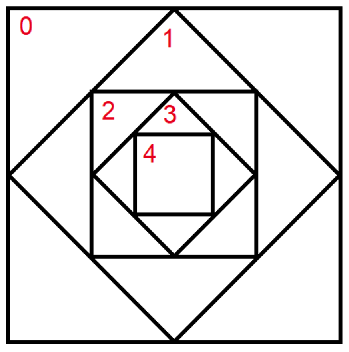
\includegraphics[scale=0.6]{./pics/A.png}}

由於Sana是一個很調皮的小孩,很喜歡到處亂跑,有時甚至會跑出洞穴到處捉弄人,因此由Sana共鳴產生的夢想世界大小會隨著她的移動有所改變,不過根據理論推算,夢想世界的範圍會是包含洞穴與Sana的最小凸多邊形圍起來的部分。身為資深的研究員,假設Sana是一個點,給定洞穴的與Sana位置的座標是否能求出Sana夢想世界的面積大小呢?

\InputFile

輸入只有兩行。第一行有$4$個整數$x_1,y_1,x_2,y_2$,表示洞穴的對角兩點的座標,洞穴的邊與座標軸平行或垂直,第二行有兩個整數$x,y$表示Sana目前的位置

\begin{iofmt}
\begin{itemize}
	\item $x_1\leq x_2$
	\item $y_1\leq y_2$
	\item $|x,y,x_1,x_2,y_1,y_2|\leq 10000$
\end{itemize}
\end{iofmt}

\OutputFile

請輸出夢想世界的面積,輸出到小數點後第$1$位。

\Examples

\begin{example}
\exmpfile{./sample/PA.sample.in}{./sample/PA.sample.out}%
\end{example}

\end{problem}
